-	Performance gain (IPC) \\
-	LFMR, MPKI \\
-	Comparison to other Special Kernels (Lulesh)


\begin{figure}[h]%[bp]
\begin{center}
\includegraphics[width=1\linewidth]{MEMSYS22/figures/ip}
\end{center}
  \vspace{-0.1in}
\caption{Positioning of the main compute kernel of MiniAMR app in Roofline. Here the red circle indicates the $findAndRecordAllPaths$ function }
\label{fig:roof-pathfinder}
\vspace{-0.2in}
\end{figure}

\begin{figure}[h]%[bp]
\begin{center}
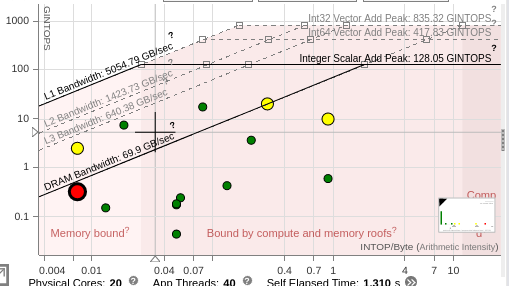
\includegraphics[width=1\linewidth]{MEMSYS22/figures/roofline/pathfinder.png}
\end{center}
  \vspace{-0.1in}
\caption{Positioning of the main compute kernel of MiniAMR app in Roofline. Here the red circle indicates the $findAndRecordAllPaths$ function }
\label{fig:roof-pathfinder}
\vspace{-0.2in}
\end{figure}

\begin{figure}[h]%[bp]
\begin{center}
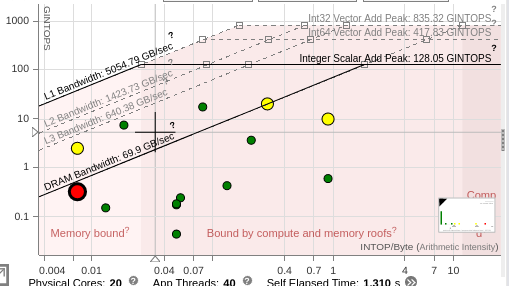
\includegraphics[width=1\linewidth]{MEMSYS22/figures/roofline/pathfinder.png}
\end{center}
  \vspace{-0.1in}
\caption{Positioning of the main compute kernel of MiniAMR app in Roofline. Here the red circle indicates the $findAndRecordAllPaths$ function }
\label{fig:roof-pathfinder}
\vspace{-0.2in}
\end{figure}


%
%\begin{figure}[t!]
%\hspace*{-9.5cm}
%\centering
%\includegraphics[width=\textwidth, height=60mm]{figure/Set1.pdf}
%%\caption{ST-1.2 Configuration (floating point benchmarks): Speedup ranges from 0\% (tonto) to 7.4\% (milc), and it is 2.7\% on average.}
%\label{fig:Set1}
%\end{figure}
%
%
%\begin{figure}[htbp]
%  
%\centering
%\includegraphics[width=\textwidth, height=60mm]{figure/Set2.pdf}
%%\caption{ST-1.2 Configuration (floating point benchmarks): Speedup ranges from 0\% (tonto) to 7.4\% (milc), and it is 2.7\% on average.}
%\label{fig:Set2}
%\end{figure}
%
%
%\begin{figure*}[t!]
%\centering
%\includegraphics[width=\textwidth, height=60mm]{figure/Set3.pdf}
%%\caption{ST-1.2 Configuration (floating point benchmarks): Speedup ranges from 0\% (tonto) to 7.4\% (milc), and it is 2.7\% on average.}
%\label{fig:Set3}
%\end{figure*}
%
%%\vspace{5cm}
%\newpage
%
%\begin{figure}[H]
%\centering
%\includegraphics[width=\textwidth, height=60mm]{figure/Set4.pdf}
%%\caption{ST-1.2 Configuration (floating point benchmarks): Speedup ranges from 0\% (tonto) to 7.4\% (milc), and it is 2.7\% on average.}
%\label{fig:Set4}
%\end{figure}








